%%%%%%%%%%%%%%%%%%%%%%%%%%%%%%%%%%%%%%%%%%%
%
% From a template maintained at https://github.com/jamesrobertlloyd/cbl-tikz-poster
%
%%%%%%%%%%%%%%%%%%%%%%%%%%%%%%%%%%%%%%%%%%%


\documentclass[portrait,a0b,final,a4resizeable]{include/a0poster}


\usepackage{multicol}
\usepackage{color}
\usepackage{morefloats}
\usepackage[pdftex]{graphicx}
\usepackage{rotating}
\usepackage{amsmath, amsthm, amssymb, bm}
\usepackage{array}
\usepackage{booktabs}
\usepackage{multirow}
\usepackage{hyperref}
\usepackage{include/picins}
\usepackage{tikz}
\usetikzlibrary{shapes.geometric,arrows,chains,matrix,positioning,scopes,calc}
\tikzstyle{mybox} = [draw=white, rectangle]
\definecolor{darkblue}{rgb}{0,0.08,0.45}
\definecolor{blue}{rgb}{0,0,1}
\usepackage{dsfont}
\usepackage[margin=0.25in]{geometry}
\usepackage{fp}

%%%%%%%%%%%%%%%%%%%%%%%%%%%%%%%%%%%%%%%%%%%
%
% myfig
%
% \myfig - replacement for \figure
% necessary, since in multicol-environment 
% \figure won't work        
%                 
%%%%%%%%%%%%%%%%%%%%%%%%%%%%%%%%%%%%%%%%%%%

\newcommand{\myfig}[3][0]{
\begin{center}
  \vspace{1.5cm}
  \includegraphics[width=#3\hsize,angle=#1]{#2}
  \nobreak\medskip
\end{center}}

%%%%%%%%%%%%%%%%%%%%%%%%%%%%%%%%%%%%%%%%%%%
%
% mycaption                
%
% \mycaption - replacement for \caption
% necessary, since in multicol-environment \figure and
% therefore \caption won't work
%
%%%%%%%%%%%%%%%%%%%%%%%%%%%%%%%%%%%%%%%%%%%

%\newcounter{figure}
\setcounter{figure}{1}
\newcommand{\mycaption}[1]{
  \vspace{0.5cm}
  \begin{quote}
    {{\sc Figure} \arabic{figure}: #1}
  \end{quote}
  \vspace{1cm}
  \stepcounter{figure}
}

%%%%%%%%%%%%%%%%%%%%%%%%%%%%%%%%%%%%%%%%%%%
%
% Some standard colours
%
%%%%%%%%%%%%%%%%%%%%%%%%%%%%%%%%%%%%%%%%%%%

\definecolor{camlightblue}{rgb}{0.601 , 0.8, 1}
\definecolor{camdarkblue}{rgb}{0, 0.203, 0.402}
\definecolor{camred}{rgb}{1, 0.203, 0}
\definecolor{camyellow}{rgb}{1, 0.8, 0}
\definecolor{lightblue}{rgb}{0, 0, 0.80}
\definecolor{white}{rgb}{1, 1, 1}
\definecolor{whiteblue}{rgb}{0.80, 0.80, 1}

%%%%%%%%%%%%%%%%%%%%%%%%%%%%%%%%%%%%%%%%%%%
%
% Some look and feel definitions
%
%%%%%%%%%%%%%%%%%%%%%%%%%%%%%%%%%%%%%%%%%%%

\setlength{\columnsep}{0.03\textwidth}
\setlength{\columnseprule}{0.0018\textwidth}
\setlength{\parindent}{0.0cm}

%%%%%%%%%%%%%%%%%%%%%%%%%%%%%%%%%%%%%%%%%%%
%
% \mysection - replacement for \section*
% 
% Puts a pretty box around some text
% TODO - any other thoughts for what this box should look like
%
%%%%%%%%%%%%%%%%%%%%%%%%%%%%%%%%%%%%%%%%%%%

\tikzstyle{mysection} = [rectangle, 
			draw=none, 
			shade, 
			outer color=camlightblue!30,
			inner color=camlightblue!30,
			text width=0.965\columnwidth,
			text centered,
			rounded corners=20pt,
			minimum height=0.09\columnwidth]

\newcommand{\mysection}[1]
{
\begin{center}
  \begin{tikzpicture}
    \node[mysection] {\sffamily\bfseries\LARGE#1};
  \end{tikzpicture}
\end{center}
}

%%%%%%%%%%%%%%%%%%%%%%%%%%%%%%%%%%%%%%%%%%%
%
% Set the font
%
% TODO - Not sure what a canonical choice is - feel free to modify
%
%%%%%%%%%%%%%%%%%%%%%%%%%%%%%%%%%%%%%%%%%%%

\renewcommand{\familydefault}{cmss}
\sffamily

%%%%%%%%%%%%%%%%%%%%%%%%%%%%%%%%%%%%%%%%%%%%%%%%%%%%
%%%               Background                     %%%
%%%%%%%%%%%%%%%%%%%%%%%%%%%%%%%%%%%%%%%%%%%%%%%%%%%%

\newcommand{\background}[3]{
  %\definecolor{cgradbegin}{#1}
  %\definecolor{cgradend}{#2}
 % \psframe[fillstyle=gradient,gradend=cgradend,
 % gradbegin=cgradbegin,gradmidpoint=#3](0.,0.)(1.\textwidth,-1.\textheight)
}




%%%%%%%%%%%%%%%%%%%%%%%%%%%%%%%%%%%%%%%%%%%%%%%%%%%%
%%%                pcolumn                       %%%
%%%%%%%%%%%%%%%%%%%%%%%%%%%%%%%%%%%%%%%%%%%%%%%%%%%%

\newenvironment{pcolumn}[1]{
  \begin{minipage}{#1\textwidth}
  \begin{center}
}{
  \end{center}
  \end{minipage}
}



%%%%%%%%%%%%%%%%%%%%%%%%%%%%%%%%%%%%%%%%%%%%%%%%%%%%
%%%                pbox                          %%%
%%%%%%%%%%%%%%%%%%%%%%%%%%%%%%%%%%%%%%%%%%%%%%%%%%%%

\definecolor{lcolor}{rgb}{0, 0, 0.80}
\definecolor{gcolor1}{rgb}{1, 1, 1}
\definecolor{gcolor2}{rgb}{.80, .80, 1}

  % \def\fc{fillcolor}
  % \def\getfc #1=#2\par{\def\ffc{#1} \ifx\ffc\fc #2\fi} 
  % \def\getfillcolor #1,#2\par{\getfc #1\par \getfc #2\par}

 %  \newcommand{\psshadowbox}[2]{%[2][magenta]{
%      \fbox{Input arg: #1}
%      \fbox{#1} 
%      \fbox {\getfillcolor #1\par}
%      \def\col{\getfillcolor #1\par}
 
%      \let\coll=\col
%       \coll
 %     \colorbox{\col}{#2}
%       \mbox
   %   \coloredshadowbox{black}{\coll}{#2}
%   }

\newcommand{\pbox}[4]{
%\psshadowbox[#3]{
%\fbox{
\mbox{
\begin{minipage}[t][#2][t]{#1}
#4
\end{minipage}
}%}
}

%%%%%%%%%%%%%%%%%%%%%%%%%%%%%%%%%%%%%%%%%%%
%
% Poster environment
%
% Centres everything and can be used to define the width of the content
%
%%%%%%%%%%%%%%%%%%%%%%%%%%%%%%%%%%%%%%%%%%%

\newenvironment{poster}{
  \begin{center}
  \begin{minipage}[c]{\textwidth}
}{
  \end{minipage}
  \end{center}
}

\def\newarrow{\mbox{\begin{tikzpicture}
             \useasboundingbox{(-3pt,-4.5pt) rectangle (19pt,1pt)};
             \draw[->] (0,-0.07)--(17pt,-0.07);\end{tikzpicture}}}



\usepackage{include/preamble}


% Custom notation
\newcommand{\fdeep}{\vf^{(1:L)}}
\newcommand{\flast}{\vf^{(L)}}
\newcommand{\Jx}{J_{\vx \rightarrow \vy}}
\newcommand{\Jxx}{J_{\vx \rightarrow \vy}(\vx)}
\newcommand{\Jy}{J_{\vy \rightarrow \vx}}
\newcommand{\Jyy}{J_{\vy \rightarrow \vx}(\vy)}
\newcommand{\detJyy}{ \left| J_{\vy \rightarrow \vx}(\vy) \right|}






\newcommand\transpose{{\textrm{\tiny{\sf{T}}}}}
\newcommand{\note}[1]{}
\newcommand{\hlinespace}{~\vspace*{-0.15cm}~\\\hline\\\vspace*{0.15cm}}
\newcommand{\embeddingletter}{g}
\newcommand{\bo}{{\sc bo}}
%\newcommand{\gp}{{\sc gp}}
\newcommand{\agp}{Arc \gp}





%\newcommand{\data}{\left\{\mathbf{x}_n, y_n\right\}_{n=1}^N}
%\newcommand{\X}{ \left\{\mathbf{x}_n \right\}_{n=1}^N }
%\newcommand{\y}{ \left\{y_n\right\}_{n=1}^N }

\newcommand{\D}{\mathcal{D}}
\newcommand{\X}{\mathbf{X}}
\newcommand{\y}{y}
\newcommand{\data} {\X, \y}
\newcommand{\x}{\mathbf{x}}
\newcommand{\f}{\mathit{f}}

%\newcommand{\candidates} {\left\{X_c\right\}_{c=1}^C}
% starting points/presets
%\newcommand{\starts} {\left\{X_s\right\}_{s=1}^S}
%\newcommand{\levels}{\left\{y_d\right\}_{d=1}^L}
%\newcommand{\lengthScales}{\left\{ \mathbf{l}_l \right\}_{l=1}^{M}}

\newcommand{\candidates} {\mathbf{X}_c}
\newcommand{\starts}{\mathbf{X}_s}
\newcommand{\levels}{\mathbf{y}_d}
\newcommand{\lengthScales}{\mathbf{L}_l}

%\newcommand{\gp}{\mathcal{GP}}
\newcommand{\fx}{ f(\mathbf{x}) }
%\newcommand{\k}{ \mathbf{k} }
%\newcommand{\K}{ \mathbf{K} }
\newcommand{\U}{\mathcal{U}}
\newcommand{\E}{\mathbf{E}}





\begin{document}


\begin{poster}

% Potentially add some space at the top of the poster
%\vspace{0\baselineskip}


%%% Header
\begin{center}
\begin{pcolumn}{1.03}

\newcommand{\logowidth}{0.099\textwidth}  % width mauna decomp
\pbox{0.99\textwidth}{}{linewidth=2mm,framearc=0.3,linecolor=camdarkblue,fillstyle=gradient,gradangle=0,gradbegin=white,gradend=white,gradmidpoint=1.0,framesep=1em}{
%
%%% Cambridge Logo
\begin{minipage}[c]{\logowidth}
  \begin{center}
%    
\includegraphics[width=6cm]{badges/University_Crest}
 %   \vspace{.1in}
  %  
\includegraphics[width=6cm]{badges/unicamtext.pdf}
  \end{center}
\end{minipage}
%
%%% Title
\begin{minipage}[c][9cm][c]{0.76\textwidth}
  \begin{center}
    {\sffamily \VeryHuge \textbf{Avoiding Pathologies in Very Deep Networks}}\\[10mm]
    {\huge\sffamily \Huge David Duvenaud, Oren Rippel, Ryan Adams, Zoubin Ghahramani\\[7.5mm]
    %\texttt{\{ti242, dkd23, zoubin\}@cam.ac.uk}
    }
  \end{center}
\end{minipage}
%
%
% Harvard logo
\begin{minipage}[c]{\logowidth}
  \begin{flushright}
   % 
\includegraphics[width=8cm,trim=2em 0em 2em 2em, clip]{badges/harvard}
  \end{flushright}
\end{minipage}
%
}
\end{pcolumn}
\end{center}

\vspace*{0.5cm}

\large


%%%%%%%%%%%%%%%%%%%%%%%%%%%%%%%%%%%%%%%%%%%%%%%%%%%%%%%%%%%%%%%%%%%%%%
%%% Beginning of Document
%%%%%%%%%%%%%%%%%%%%%%%%%%%%%%%%%%%%%%%%%%%%%%%%%%%%%%%%%%%%%%%%%%%%%%

\Large


\begin{multicols}{2}


%\mysection{Abstract}
%\begin{itemize}
%	\item We analyze deep Gaussian processes, a type of infinitely-wide, deep neural net.
%	\item We study distributions of deep GPs and a find a pathology, then show a simple fix.
%	\item We also derive kernels corresponding to infinitely deep nets.
%\end{itemize}
%\vspace{0.5in}

\mysection{Nonparametric Priors on Deep Nets}

%\begin{figure*}
%\def\layersep{1.14cm}
\def\nodesep{.75cm}
\def\nodesize{.35cm}

\newcommand{\numdims}[0]{3}
\newcommand{\numhidden}[0]{4}

\begin{tabular}{c|c|c}
\hspace{-1cm}
\begin{tikzpicture}[shorten >=1pt,->,draw=black!50, node distance=\layersep]
    \tikzstyle{every pin edge}=[<-,shorten <=1pt]
    \tikzstyle{neuron}=[circle,fill=black!25,minimum size=17pt,inner sep=0pt]
    \tikzstyle{input neuron}=[neuron, fill=green!50];
    \tikzstyle{output neuron}=[neuron, fill=red!50];
    \tikzstyle{hidden neuron}=[neuron, fill=blue!50];
    \tikzstyle{annot} = [text width=4em, text centered]

    % Draw the input layer nodes
    \foreach \name / \y in {1,...,\numdims}
    % This is the same as writing \foreach \name / \y in {1/1,2/2,3/3,4/4}
        \node[input neuron, minimum size=\nodesize
        %, pin=left:Input \#\y
        ] (I-\name) at (0,-\nodesep*\y) {};

    % Draw the hidden layer nodes
    \foreach \name / \y in {1,...,\numhidden}
        \path[yshift=0.5cm]
            node[hidden neuron, minimum size=\nodesize] (H-\name) at (\layersep,-\nodesep*\y) {};

    % Draw the output layer node
    \foreach \name / \y in {1,...,\numdims}
    	\node[output neuron, minimum size=\nodesize
    	%,pin={[pin edge={->}]right:Output }
    	] (O-\name) at (2*\layersep,-\nodesep*\y) {};

    % Connect every node in the input layer with every node in the
    % hidden layer.
    \foreach \source in {1,...,\numdims}
        \foreach \dest in {1,...,\numhidden}
            \path (I-\source) edge (H-\dest);

    % Connect every node in the hidden layer with the output layer
    \foreach \source in {1,...,\numhidden}
        \foreach \dest in {1,...,\numdims}
    	    \path (H-\source) edge (O-\dest);

    % Annotate the layers
    \node[annot,above of=H-1, node distance=0.7cm] (hl) {Hidden};
    \node[annot,left of=hl] {Input};
    \node[annot,right of=hl] {Output};
\end{tikzpicture}
\hspace{-0.4cm}
&
\hspace{-0.4cm}
\begin{tikzpicture}[shorten >=1pt,->,draw=black!50, node distance=\layersep]
    \tikzstyle{every pin edge}=[<-,shorten <=1pt]
    \tikzstyle{neuron}=[circle,fill=black!25,minimum size=17pt,inner sep=0pt]
    \tikzstyle{input neuron}=[neuron, fill=green!50];
    \tikzstyle{output neuron}=[neuron, fill=red!50];
    \tikzstyle{hidden neuron}=[neuron, fill=blue!50];
    \tikzstyle{annot} = [text width=4em, text centered]

    % Draw the input layer nodes
    \foreach \name / \y in {1,...,\numdims}
    % This is the same as writing \foreach \name / \y in {1/1,2/2,3/3,4/4}
        \node[input neuron, minimum size=\nodesize
        %, pin=left:Input \#\y
        ] (I-\name) at (0,-\nodesep*\y) {};

    % Draw the hidden layer nodes
    \foreach \name / \y in {1,...,\numhidden}
        \path[yshift=0.5cm]
            node[hidden neuron, minimum size=\nodesize] (H-\name) at (\layersep,-\nodesep*\y) {};

    % Draw the hidden layer nodes
    \foreach \name / \y in {1,...,\numhidden}
        \path[yshift=0.5cm]
            node[hidden neuron, minimum size=\nodesize] (H2-\name) at (2*\layersep,-\nodesep*\y) {};


    % Draw the output layer node
    \foreach \name / \y in {1,...,\numdims}
    	\node[output neuron, minimum size=\nodesize
    	%,pin={[pin edge={->}]right:Output }
    	] (O-\name) at (3*\layersep,-\nodesep*\y) {};

    % Connect every node in the input layer with every node in the
    % hidden layer.
    \foreach \source in {1,...,\numdims}
        \foreach \dest in {1,...,\numhidden}
            \path (I-\source) edge (H-\dest);
            
    \foreach \source in {1,...,\numhidden}
        \foreach \dest in {1,...,\numhidden}
            \path (H-\source) edge (H2-\dest);            

    % Connect every node in the hidden layer with the output layer
    \foreach \source in {1,...,\numhidden}
        \foreach \dest in {1,...,\numdims}
    	    \path (H2-\source) edge (O-\dest);

    % Annotate the layers
    \node[annot,above of=H-1, node distance=0.7cm] (hl) {Hidden};
    \node[annot,above of=H2-1, node distance=0.7cm] (hl2) {Hidden};    
    \node[annot,left of=hl] {Input};
    \node[annot,right of=hl2] {Output};
\end{tikzpicture}
\hspace{-0.4cm}
&
\hspace{-0.4cm}
\begin{tikzpicture}[shorten >=1pt,->,draw=black!50, node distance=\layersep]
    \tikzstyle{every pin edge}=[<-,shorten <=1pt]
    \tikzstyle{neuron}=[circle,fill=black!25,minimum size=17pt,inner sep=0pt]
    \tikzstyle{input neuron}=[neuron, fill=green!50];
    \tikzstyle{output neuron}=[neuron, fill=red!50];
    \tikzstyle{hidden neuron}=[neuron, fill=blue!50];
    \tikzstyle{annot} = [text width=4em, text centered]

    % Draw the input layer nodes
    \foreach \name / \y in {1,...,\numdims}
    % This is the same as writing \foreach \name / \y in {1/1,2/2,3/3,4/4}
        \node[input neuron, minimum size=\nodesize
        %, pin=left:Input \#\y
        ] (I-\name) at (0,-\nodesep*\y) {};

    % Draw the hidden layer nodes
    \foreach \name / \y in {1,...,\numhidden}
        \path[yshift=0.5cm]
            node[hidden neuron, minimum size=\nodesize] (H-\name) at (\layersep,-\nodesep*\y) {};

    % Draw the hidden layer nodes
    \foreach \name / \y in {1,...,\numhidden}
        \path[yshift=0.5cm]
            node[hidden neuron, minimum size=\nodesize] (H2-\name) at (3*\layersep,-\nodesep*\y) {};

    % Draw the output layer node
    \foreach \name / \y in {1,...,\numdims}
    	\node[output neuron, minimum size=\nodesize
    	%,pin={[pin edge={->}]right:Output }
    	] (O1-\name) at (2*\layersep,-\nodesep*\y) {};

    % Draw the output layer node
    \foreach \name / \y in {1,...,\numdims}
    	\node[output neuron, minimum size=\nodesize
    	%,pin={[pin edge={->}]right:Output }
    	] (O2-\name) at (4*\layersep,-\nodesep*\y) {};

    % Connect every node in the input layer with every node in the
    % hidden layer.
    \foreach \source in {1,...,\numdims}
        \foreach \dest in {1,...,\numhidden}
            \path (I-\source) edge (H-\dest);
            
    \foreach \source in {1,...,\numhidden}
        \foreach \dest in {1,...,\numdims}
            \path (H-\source) edge (O1-\dest);         
            
    \foreach \source in {1,...,\numdims}
        \foreach \dest in {1,...,\numhidden}
            \path (O1-\source) edge (H2-\dest);                

    % Connect every node in the hidden layer with the output layer
    \foreach \source in {1,...,\numhidden}
        \foreach \dest in {1,...,\numdims}
    	    \path (H2-\source) edge (O2-\dest);

    % Annotate the layers
    \node[annot,above of=H-1, node distance=0.7cm] (hl) {Hidden};
    \node[annot,left of=hl] {Input};
    \node[annot,right of=hl] {$f^1(\vx)$};
    \node[annot,above of=H2-1, node distance=0.7cm] (hl2) {Hidden};
    \node[annot,right of=hl2] {$f^{1:2}(\vx)$};
\end{tikzpicture} \\
\hspace{-0.5cm} Single-layer NN, or \gp{}& 2-Hidden layer NN & \hspace{-0.3cm} Two-layer \gp{} model: $\vy = f_2(f_1(\vx))$
\end{tabular}

%\caption{Comparing architectures.
%In the deep \gpt{} models, there are two possible meanings for the hidden units.  
%We can consider every other layer to be a linear combination of an infinite number of parametric hidden units. Alternatively, we can integrate out the hidden layers, and consider the deep \gpt{} to be a neural network with a finite number of hidden units, each with a different non-parametric activation function.}
%\label{fig:architectures}
%\end{figure*}

\vspace{0.5in} 

%\begin{tabular}{cc}
%\begin{minipage}[c]{0.7\columnwidth}

Deep \gp{}s are compositions of functions, each $f^{(\ell)} \simind \GPt{0}{k(\vx, \vx')}$. 
\begin{align*}
\vf^{(1:L)}(\vx) = \vf^{(L)}(\vf^{(L-1)}(\dots \vf^{(2)}(\vf^{(1)}(\vx)) \dots))
\end{align*}
%

Can be derived as either
\begin{enumerate}
	\item  neural nets with nonparametric activation functions
    \item  neural nets with infintely-many parametric hidden nodes
\end{enumerate}



\newlength{\arrowsize}  
\pgfarrowsdeclare{biggertip}{biggertip}{  
  \setlength{\arrowsize}{10pt}  
  \addtolength{\arrowsize}{2\pgflinewidth}  
  \pgfarrowsrightextend{0}  
  \pgfarrowsleftextend{-5\arrowsize}  
}{  
  \setlength{\arrowsize}{1pt}  
  \addtolength{\arrowsize}{\pgflinewidth}  
  \pgfpathmoveto{\pgfpoint{-5\arrowsize}{4\arrowsize}}  
  \pgfpathlineto{\pgfpointorigin}  
  \pgfpathlineto{\pgfpoint{-5\arrowsize}{-4\arrowsize}}  
  \pgfusepathqstroke  
} 




%
\def\layersep{8cm}
\def\nodesep{3.3cm}
\def\halfshift{1.65cm}
\def\nodesize{2.5cm}

\newcommand{\numdims}[0]{3}
\newcommand{\numhidden}[0]{4}
\newcommand{\upnodedist}[0]{2.3cm}

\newcommand{\neuronfunc}[2]{
\FPeval{\result}{clip(#1+#2)}
%
\null\hspace*{-0.5cm}\includegraphics[width=1.9cm, clip, trim=10mm 0mm 10mm 0mm]{../../figures/two-d-draws/sqexp-draw-\result}
%\end{pgfonlayer}
}


\begin{tabular}{c}
\begin{tikzpicture}[draw=black, node distance=\layersep]
    \tikzstyle{interarrows}=[->, ultra thick, -biggertip, black!50, line width = 2pt, shorten >= -0cm, shorten <= -0cm]
    \tikzstyle{neuron}=[circle, draw = black, inner sep=-0pt, line width = 2pt]
    \tikzstyle{input neuron}=[neuron, minimum size=\nodesize];
    \tikzstyle{output neuron}=[neuron, minimum size=\nodesize];
    \tikzstyle{hidden neuron}=[neuron, minimum size=\nodesize];
    \tikzstyle{annot} = [text width=4em, text centered]

    % Draw the input layer nodes
    \foreach \name / \y in {1,...,\numdims}
        \node[input neuron] (I-\name) at (0,-\nodesep*\y) {$x_\y$};

    % Draw the hidden layer nodes
    \foreach \name / \y in {1,...,\numhidden}
        \path[yshift=\halfshift] node[hidden neuron] (H-\name) at (\layersep,-\nodesep*\y) { \neuronfunc{\y}{0}};

    % Draw the hidden layer nodes
    \foreach \name / \y in {1,...,\numhidden}
        \path[yshift=\halfshift] node[hidden neuron] (H2-\name) at (2*\layersep,-\nodesep*\y) {\neuronfunc{\y}{4}};

    % Draw the output layer node
    \foreach \name / \y in {1,...,\numdims}
    	\node[output neuron] (O-\name) at (3*\layersep,-\nodesep*\y) {\neuronfunc{\y}{8}};

    % Connect every node in the input layer with every node in the hidden layer.
    \foreach \source in {1,...,\numdims}
        \foreach \dest in {1,...,\numhidden}
            \path (I-\source) edge[interarrows] (H-\dest);
            
    \foreach \source in {1,...,\numhidden}
        \foreach \dest in {1,...,\numhidden}
            \path (H-\source) edge[interarrows] (H2-\dest);            

    % Connect every node in the hidden layer with the output layer
    \foreach \source in {1,...,\numhidden}
        \foreach \dest in {1,...,\numdims}
    	    \path (H2-\source) edge[interarrows] (O-\dest);

    % Annotate the layers
    \node[annot,above of=I-1, node distance=\upnodedist] {Inputs};
    \node[annot,below of=I-\numdims, node distance=\upnodedist] {$\vx$};    
    \node[annot,above of=H-1, node distance=\upnodedist, text width = 7cm] {Hidden Layer};
    \node[annot,above of=H2-1, node distance=\upnodedist, text width = 7cm] {Hidden Layer};
    \node[annot,below of=H-\numhidden, node distance=2.5cm, text width = 7cm] {$\vf^{(1)}(\vx)$};
    \node[annot,below of=H2-\numhidden, node distance=2.5cm, text width = 7cm] {$\vf^{(2)}(\vf^{(1)}(\vx))$};
    \node[annot,above of=O-1, node distance=\upnodedist] {Outputs};
    \node[annot,below of=O-\numdims, node distance=2.5cm, text width = 7cm] {$\vy$};
\end{tikzpicture}
\end{tabular}




\def\layersep{8cm}
\def\nodesep{3.3cm}
\def\halfshift{1.65cm}
\def\nodesize{2.5cm}

\newcommand{\numdims}[0]{3}
\newcommand{\numhidden}[0]{4}
\newcommand{\upnodedist}[0]{2.3cm}

\newcommand{\neuronfunc}[2]{
\FPeval{\result}{clip(#1+#2)}
%
\null\hspace*{-0.5cm}\includegraphics[width=1.9cm, clip, trim=10mm 0mm 10mm 0mm]{../../figures/two-d-draws/sqexp-draw-\result}
%\end{pgfonlayer}
}


\begin{tabular}{c}
\begin{tikzpicture}[draw=black, node distance=\layersep]
    \tikzstyle{interarrows}=[->, ultra thick, -biggertip, black!50, line width = 2pt, shorten >= -0cm, shorten <= -0cm]
    \tikzstyle{neuron}=[circle, draw = black, inner sep=-0pt, line width = 2pt]
    \tikzstyle{input neuron}=[neuron, minimum size=\nodesize];
    \tikzstyle{output neuron}=[neuron, minimum size=\nodesize];
    \tikzstyle{hidden neuron}=[neuron, minimum size=\nodesize];
    \tikzstyle{annot} = [text width=4em, text centered]

    % Draw the input layer nodes
    \foreach \name / \y in {1,...,\numdims}
        \node[input neuron] (I-\name) at (0,-\nodesep*\y) {$x_\y$};

    % Draw the hidden layer nodes
    \foreach \name / \y in {1,...,\numhidden}
        \path[yshift=\halfshift] node[hidden neuron] (H-\name) at (\layersep,-\nodesep*\y) { \neuronfunc{\y}{0}};

    % Draw the hidden layer nodes
    \foreach \name / \y in {1,...,\numhidden}
        \path[yshift=\halfshift] node[hidden neuron] (H2-\name) at (2*\layersep,-\nodesep*\y) {\neuronfunc{\y}{4}};

    % Draw the output layer node
    \foreach \name / \y in {1,...,\numdims}
    	\node[output neuron] (O-\name) at (3*\layersep,-\nodesep*\y) {\neuronfunc{\y}{8}};

    % Connect every node in the input layer with every node in the hidden layer.
    \foreach \source in {1,...,\numdims}
        \foreach \dest in {1,...,\numhidden}
            \path (I-\source) edge[interarrows] (H-\dest);
            
    \foreach \source in {1,...,\numhidden}
        \foreach \dest in {1,...,\numhidden}
            \path (H-\source) edge[interarrows] (H2-\dest);            

    % Connect every node in the hidden layer with the output layer
    \foreach \source in {1,...,\numhidden}
        \foreach \dest in {1,...,\numdims}
    	    \path (H2-\source) edge[interarrows] (O-\dest);

    % Annotate the layers
    \node[annot,above of=I-1, node distance=\upnodedist] {Inputs};
    \node[annot,below of=I-\numdims, node distance=\upnodedist] {$\vx$};    
    \node[annot,above of=H-1, node distance=\upnodedist, text width = 7cm] {Hidden Layer};
    \node[annot,above of=H2-1, node distance=\upnodedist, text width = 7cm] {Hidden Layer};
    \node[annot,below of=H-\numhidden, node distance=2.5cm, text width = 7cm] {$\vf^{(1)}(\vx)$};
    \node[annot,below of=H2-\numhidden, node distance=2.5cm, text width = 7cm] {$\vf^{(2)}(\vf^{(1)}(\vx))$};
    \node[annot,above of=O-1, node distance=\upnodedist] {Outputs};
    \node[annot,below of=O-\numdims, node distance=2.5cm, text width = 7cm] {$\vy$};
\end{tikzpicture}
\end{tabular}






























%\subsection*{One-dimensional asymptotics}
%\begin{itemize}
%\item Derivative size distribution approaches log-normal: small almost everywhere, with large jumps.
%\end{itemize}

%\newcommand{\onedsamplepic}[1]{
%\hspace{-0.2in}
%\includegraphics[trim=2mm 2mm 2mm 6.4mm, clip, width=0.25\columnwidth]{../figures/1d_samples/latent_seed_0_1d_large/layer-#1}} 
%\newcommand{\onedsamplepiccon}[1]{
%\hspace{-0.2in}
%\includegraphics[trim=2mm 2mm 2mm 6.4mm, clip, width=0.25\columnwidth]{../figures/1d_samples/latent_seed_0_1d_large_connected/layer-#1}} 

%\begin{tabular}{ccc}
%One-layer \gp{} & 5-Layer Composition & 10-Layer Composition \\
%\onedsamplepic{1} & \onedsamplepic{5} & \onedsamplepic{10}
%\end{tabular}





\end{multicols}



\end{poster}

\end{document}



 
\mysection{Random Deep Nets Capture Few Degrees of Freedom}

Sampled mappings illustrate properties of this prior on functions:
\vspace{0.3in}

\newcommand{\mappic}[1]{\hspace{-0.05in}\includegraphics[width=0.24\columnwidth]{../../figures/seed-0-map/latent_coord_map_layer_#1}}
 
\newcommand{\mappiccon}[1]{\hspace{-0.05in}\includegraphics[width=0.24\columnwidth]{../../figures/seed-0-map-connected/latent_coord_map_layer_#1}}

\centering
\begin{tabular}{cccc}
Identity Map& 1 Layer & 2 Layers & 40 Layers \\
\hspace{-0.1in}
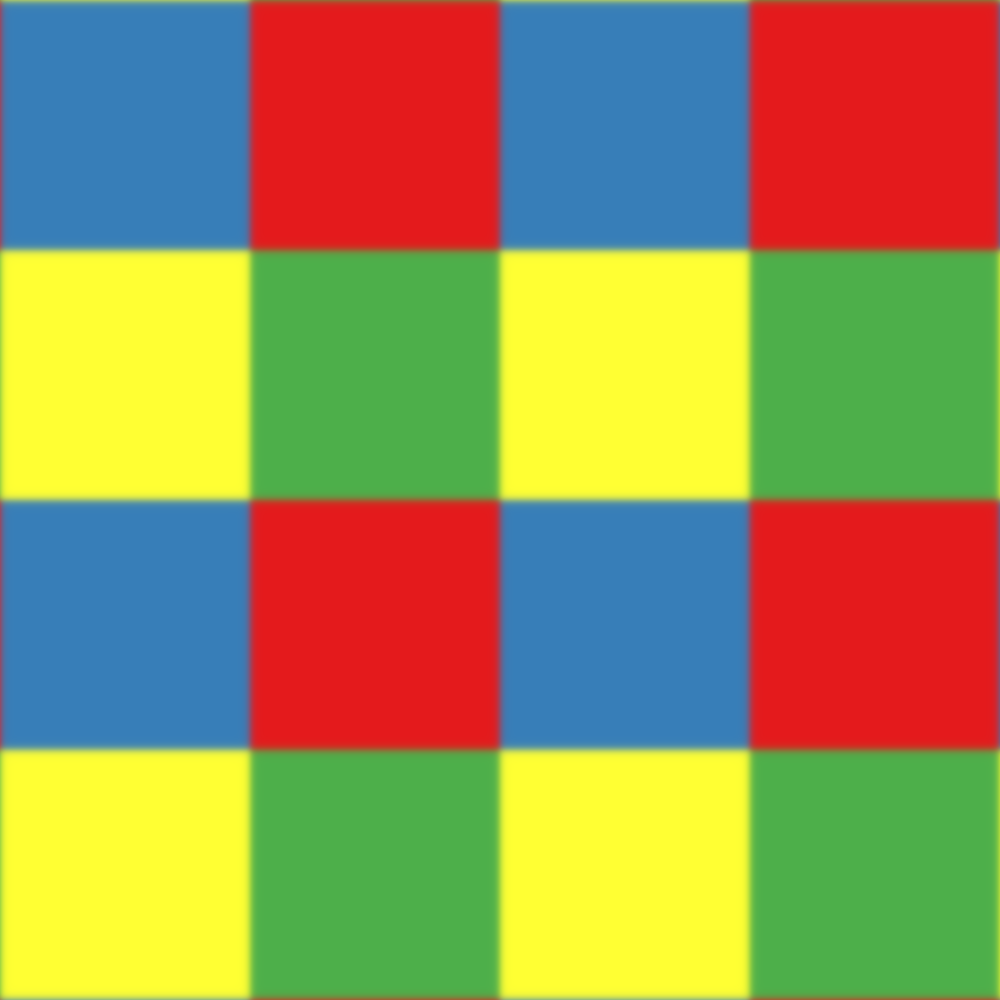
\includegraphics[width=0.24\columnwidth]{../../figures/seed-0-map/layer_0} & \mappic{1} & \mappic{10} & \mappic{40} \\
$\vy = \vx$ & $\vy = \vf^{(1)}(\vx)$ & $\vy = \vf^{(1:2)}(\vx)$ & $\vy = \vf^{(1:40)}(\vx)$
\end{tabular}



\newcommand{\gpdrawbox}[1]{
\setlength\fboxsep{0pt}
\hspace{-0.36in} 
\fbox{\hspace{-3mm}
\includegraphics[width=0.23\columnwidth]{../figures/deep_draws/deep_gp_sample_layer_#1}
\hspace{-3mm}}}

As depth increases, there is usually only one direction we can move $\vx$ to change $\vy$.

\vspace{0.5in}
A distribution warped by successive functions drawn from a \gp{} prior:
\vspace{0.5in}

\centering
\begin{tabular}{cccc}
$p(\vx)$ & $p(\vf^{(1)}(\vx))$ & $p(\vf^{(1:4)}(\vx))$ &  $p(\vf^{(1:6)}(\vx))$ \\
\hspace{-0.1in} \gpdrawbox{1} & \gpdrawbox{2} & \gpdrawbox{4} & \gpdrawbox{6} \\
\end{tabular}
As depth increases, the density concentrates along one-dimensional filaments.
\vspace{0.3in}





\mysection{Good Representations Change Along All Tangents}

\begin{tabular}{cc}
\begin{minipage}[c]{0.45\columnwidth}
\centering
\begin{tabular}{c}
Contours of a good representation \\
%\includegraphics[width=0.45\columnwidth]{figures/hidden_good} &
\begin{tikzpicture}[pile/.style={thick, ->, >=stealth'}]
    \node[anchor=south west,inner sep=0] at (0,0) {
    	\includegraphics[clip, trim = 0cm 12cm 0cm 0.0cm, width=\columnwidth]{../figures/hidden_good}
    };
    \coordinate (D) at (2.5,2.3);
    \coordinate (Do) at (4.1,0.9);
    \coordinate (Dt) at (4.44,4.2);
    
    \draw[pile] (D) -- (Dt) node[right, text width=5em] { tangent };
    \draw[pile] (D) -- (Do) node[right, text width=5em] { orthogonal };
\end{tikzpicture}
\end{tabular}

\end{minipage}
&
\begin{minipage}[c]{0.5\columnwidth}
\begin{itemize}
%\item A good latent representation is invariant in directions orthogonal to the manifold on which the data lie.  { \color{mydarkblue} (Rifai et. al., 2011)}
\item Representation $\vy = \vf(\vx)$ should capture relevant degrees of freedom of $\vx$.
\item Representation must change in directions tangent to the data manifold, to preserve information.
\end{itemize}
\end{minipage}
\end{tabular}



\mysection{Explaining the Pathology}

\newcommand{\spectrumpic}[1]{
%\hspace{-0.2in}
\includegraphics[trim=5mm 0mm 4mm 3mm, clip, width=0.425\columnwidth]{../figures/spectrum/layer-#1}} 


\begin{tabular}{cc}
\begin{minipage}[c]{0.45\columnwidth}

%{\bf Theorem}
%The Jacobian of a deep \gp{} with a product kernel is a product of independent Gaussian matrices, with each entry in each matrix being drawn independently.

\begin{itemize}
\item Jacobian of a deep \gp{} is a product of independent Gaussian matrices.%, easy to analyze.
\item Singular value spectrum shows relative size of derivatives.
\item As net deepens, one direction has much larger derivative than others.
%\item Only one direction we can move $\vx$ to change $\vy$.
\end{itemize}

%Normalized singular value spectrum of the Jacobian of a deep GP.    This implies that with high probability, there is only one effective degree of freedom in the representation being computed.  As depth increases, the distribution on singular values also becomes heavy-tailed.

\end{minipage}
&
\begin{minipage}[cc]{0.55\columnwidth}
\begin{centering}
\begin{tabular}{ccc}
2 layer SV spectrum & 6 layer SV spectrum \\
\hspace{-0.16in} \spectrumpic{2} &
\hspace{-0.16in} \spectrumpic{6} 
%2 layers & 4 layers & 6 layers
\end{tabular}
\end{centering}
\end{minipage}
\end{tabular}





\newpage








\mysection{Fixing the pathology}
\centering
%\begin{tabular}{C{0.5\columnwidth}|c}
\begin{itemize}
	\item 
	Following {\color{mydarkblue} (Neal, 1995)}, we connect the input to every layer:
\end{itemize}
%&
%\def\layersep{1.33cm}
\def\nodeseptwo{1.8cm}
%\def\nodesize{.35cm}

%\newcommand{\numdims}[0]{3}
%\newcommand{\numhidden}[0]{4}
%\newcommand{\upnodedist}[0]{0.6cm}
%\newcommand{\bardist}[0]{\hspace{-0.2cm}}

\begin{tabular}{c}
\bardist
Standard architecture: \\
\begin{tikzpicture}[draw=black!80]
    \tikzstyle{neuron}=[circle,minimum size=17pt, draw = black!80, fill = white, thick]
    \tikzstyle{input neuron}=[neuron, fill=green!50];
    \tikzstyle{output neuron}=[neuron, fill=red!50];
    \tikzstyle{hidden neuron}=[neuron, fill=blue!50];
    \tikzstyle{pile} =[thick, ->, >=stealth', shorten <=7pt, shorten >=8pt];

    % Define the input layer node
    \coordinate (I) at (0, 0);


    % Define the hidden layer nodes
    \foreach \name / \i in {1,...,\numhidden}
    {
        \coordinate (H-\name) at (\nodeseptwo * \i, 0);
    }

    % Connect every node            
    \foreach \name in {1,...,\numhidden}
    {
	 \path[pile] (I) edge (H-\name) {};
         %\path[pile] (I) edge [bend left] (H-\name) {};
    }

    \draw (I) node[neuron] {};
    \draw (I) node[below = 0.5cm]  {$\vx$};

    % Draw the hidden layer nodes
    \foreach \name / \y in {1,...,\numhidden}
    {
	\draw (H-\name) node[neuron]  {};
        \draw (H-\name) node[below = 0.34cm] {$\vf^{(\y)}(\vx)$};
    }
\end{tikzpicture} \\
\vspace{\baselineskip}
\\
Input-connected architecture: \\
\bardist
\begin{tikzpicture}[draw=black!80]
    \tikzstyle{neuron}=[circle,minimum size=17pt, draw = black!80, fill = white, thick]
    \tikzstyle{input neuron}=[neuron, fill=green!50];
    \tikzstyle{output neuron}=[neuron, fill=red!50];
    \tikzstyle{hidden neuron}=[neuron, fill=blue!50];
    \tikzstyle{pile} =[thick, ->, >=stealth', shorten <=7pt, shorten >=8pt];

    % Define the input layer node
    \coordinate (I) at (0, 0);


    % Define the hidden layer nodes
    \foreach \name / \y in {1,...,\numhidden}
    {
        \coordinate (H-\name) at (\nodeseptwo*\y, 0);
    }

    % Connect every node            
    \path[pile] (I) edge (H-1) {};
    \foreach \name in {2,...,\numhidden}
    {
	 \path[pile] (I) edge (H-\name) {};
         \path[pile] (I) edge [bend left] (H-\name) {};
    }

    \draw (I) node[neuron] {};
    \draw (I) node[below = 0.5cm]  {$\vx$};

    % Draw the hidden layer nodes
    \foreach \name / \y in {1,...,\numhidden}
    {
	\draw (H-\name) node[neuron]  {};
        \draw (H-\name) node[below = 0.34cm] {$\vf^{(\y)}(\vx)$};
    }
\end{tikzpicture} 
\end{tabular}

%\end{tabular}
%Two different architectures for deep neural networks.  The standard architecture connects each layer's outputs to the next layer's inputs.  The input-connected architecture connects also connects the original input $\vx$ to each layer.

\vspace{0.3in}

\begin{itemize}
	\item This fixes the problem:  Locally up to $D$ degrees of freedom, at any depth:
\end{itemize}
\vspace{0.3in}

\begin{tabular}{cccc}
Identity Map %$\vy = \vx$ 
& 2 connected Layers & 10 Connected Layers & 40 Connected Layers \\%\\2 Layers: $\vy = f_1(f_2(\vx))$ \\
\hspace{-0.5in} \hspace{-0.05in}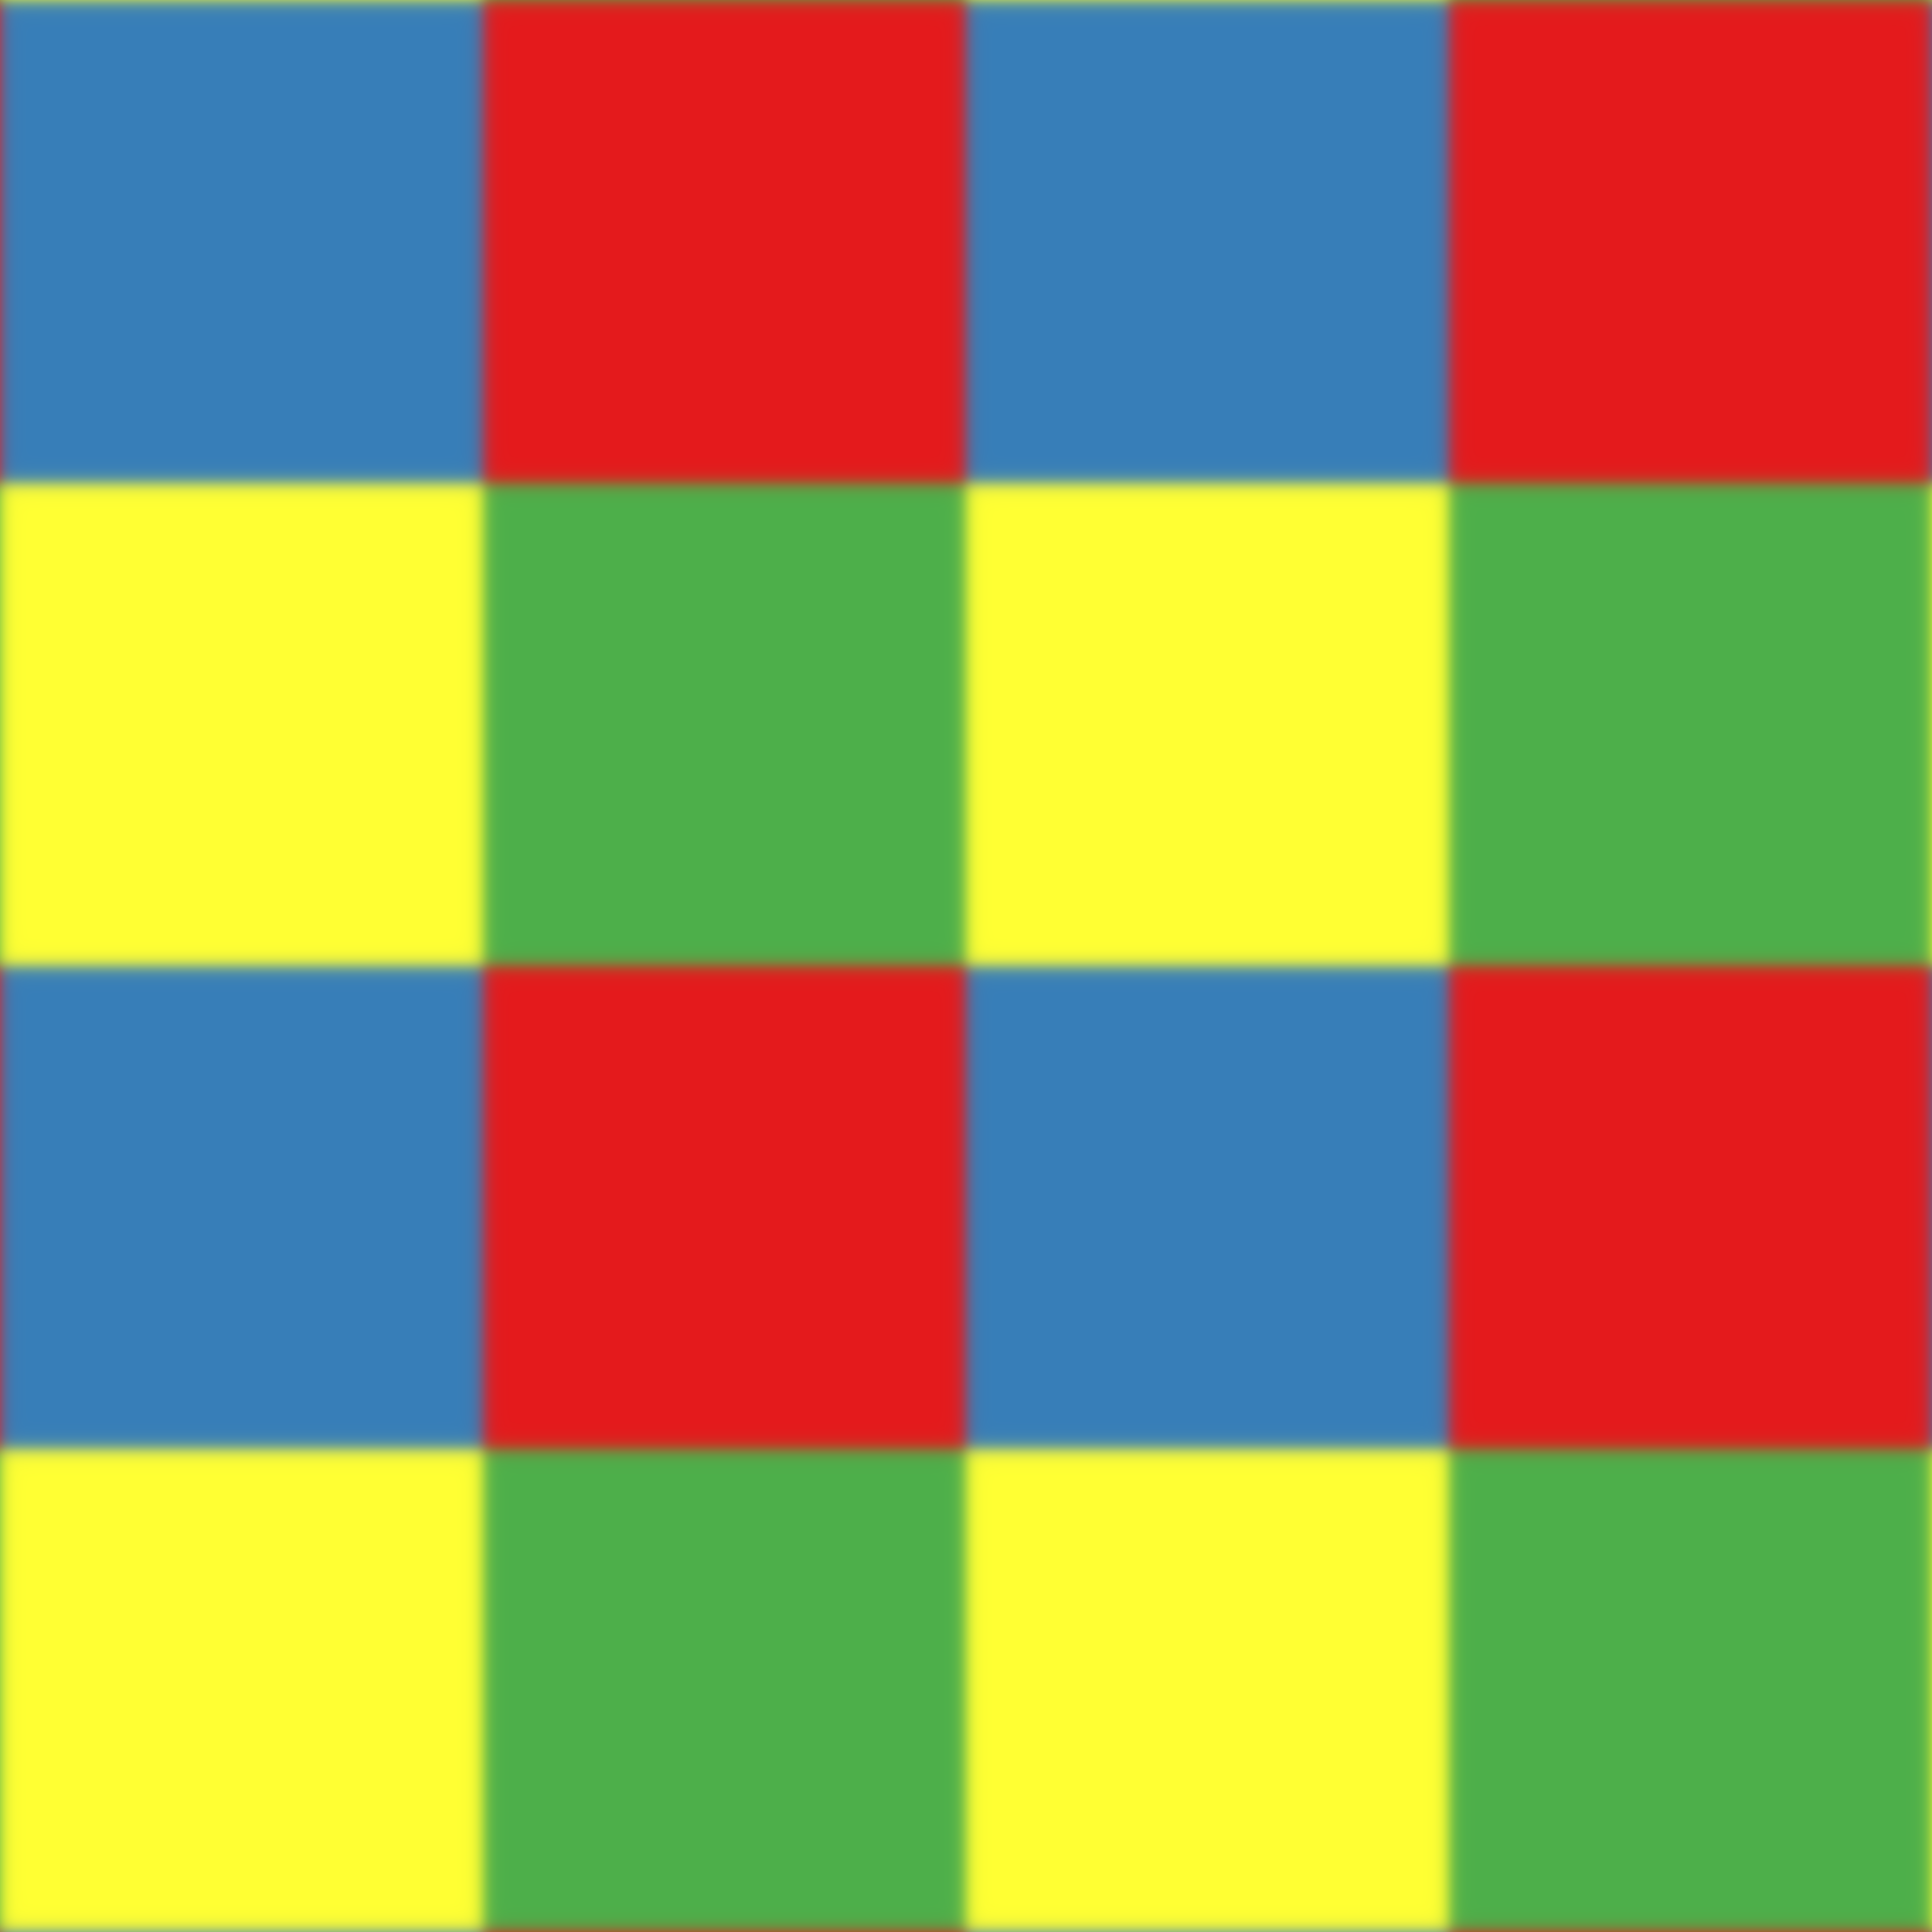
\includegraphics[width=0.24\columnwidth]{../../figures/seed-0-map-connected/layer_0} & \mappiccon{1} & \mappiccon{10} & \mappiccon{40}
%\mappic{4} & \mappic{10} & \mappic{40} \\
%4 Layers & 10 Layers & 
\end{tabular}


\newcommand{\gpdrawboxcon}[1]{
\setlength\fboxsep{0pt}
\hspace{-0.4in} 
\fbox{
\includegraphics[width=0.47\columnwidth]{../../figures/connected_deep_sample_seed_0/deep_sample_connected_layer#1}
}}

\begin{tabular}{cc}
\begin{minipage}[c]{0.45\columnwidth}
Pathology is also resolved in deep density models:  Density does not concentrate along filaments when input connects to all layers.
\end{minipage}
&
\begin{minipage}[c]{0.45\columnwidth}
\centering
\begin{tabular}{cc}
%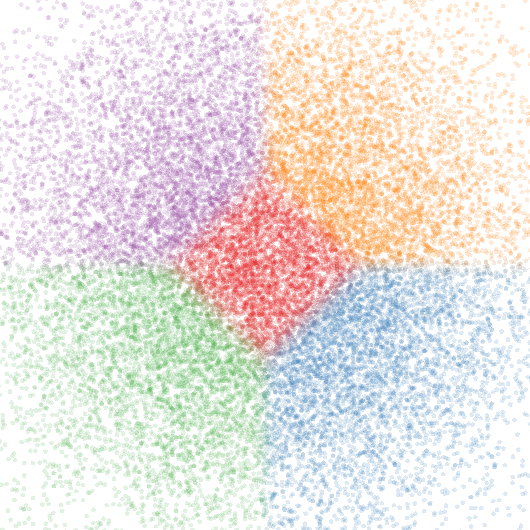
\includegraphics[width=0.3\columnwidth]{figures/deep_draws/deep_gp_sample_layer_1} &
%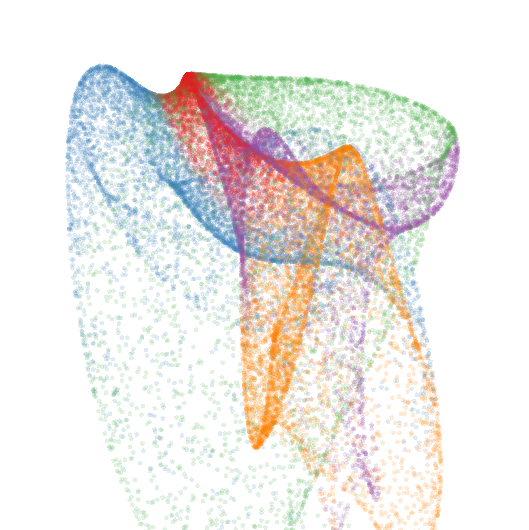
\includegraphics[width=0.3\columnwidth]{figures/deep_draws_connected/deep_sample_connected_layer2} &
%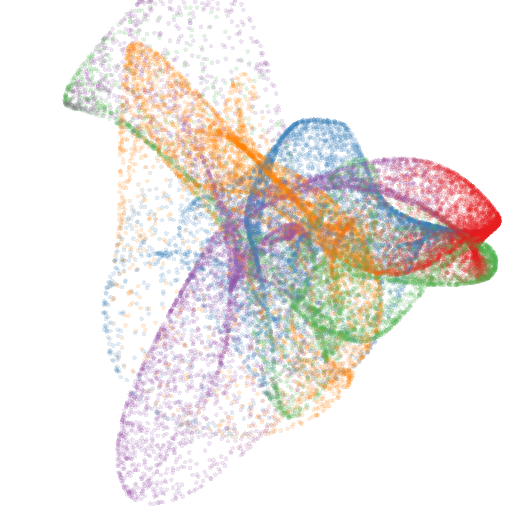
\includegraphics[width=0.3\columnwidth]{figures/deep_draws_connected/deep_sample_connected_layer3} \\
%$p(\vx)$ & $p(f_1(\vx))$ & $p(f_2(f_1(\vx), \vx))$ \\ \\
%\gpdrawboxcon{2} &
 4 Layers & 5 Layers \\
\gpdrawboxcon{4} &
\gpdrawboxcon{5}
\end{tabular}
\end{minipage}
\end{tabular}









\mysection{Infinitely Deep Kernels}

\newcommand{\feat}{\vh}

\begin{minipage}[c]{0.5\columnwidth}

\begin{itemize}
%\item Can also analyze fixed deep feature mappings:
%\item {\color{mydarkblue} (Cho, 2012) } built kernels from multiple layers of feature mappings:
\item If ${k_1(\vx, \vx') = \feat(\vx) \tra \feat(\vx')}$,

% we can also build kernel 
 ${k_2(\vx, \vx') = \feat(\feat(\vx)) \tra \feat(\feat(\vx'))}$.
%
%We can consider applying the feature transform $\Phi(\cdot)$ to the features themselves:  $\Phi_2 = \Phi(\Phi(\vx))$.  

\item Recurrent limit for squared-exp kernel: % for any set of starting features $\Phi_n(\vx)$:
%
%In this section, we take the infinite limits of these compositions, and propose a new variant.
%
%One can derive a Gaussian process as a neural network: $f(x) = {\mathbf \alpha}^T \Phi(x) = \sum_{i=i}^K \alpha_i \phi_i(x)$.  
%
%
%we derive a kernel which corresponds to arbitrarily many compositions of the feature vectors corresponding to the squared-exp kernel:
%
%\begin{align*}
%k_1(\vx, \vx') & = \exp \left( -\frac{1}{2} ||\vx - \vx'||_2^2 \right) \\
%& k_{n+1}(\vx, \vx') = \nonumber \\
%& = \exp \left( -\frac{1}{2} \left|\left| \left[ \! \begin{array}{c} \Phi_n(\vx) \\ \vx \end{array} \! \right]  - \left[ \! \begin{array}{c} \Phi_n(\vx') \\ \vx' \end{array} \! \right] \right| \right|_2^2 \right) \nonumber \\
%k_{n+1}(\vx, \vx') 
%& = \exp \left( -\frac{1}{2} \sum_i \left[ \phi_i(\vx) - \phi_i(\vx') \right]^2 -\frac{1}{2} || \vx - \vx' ||_2^2 \right) \\
%k_{n+1}(\vx, \vx') & = \exp\left ( -\frac{1}{2} \sum_i \left[ \phi_i(\vx)^2 - 2 \phi_i(\vx) \phi_i(\vx') + \phi_i(\vx')^2 \right]  -\frac{1}{2} || \vx - \vx' ||_2^2 \right) \\
%k_2(\vx, \vx') & = \exp \left( -\frac{1}{2} \left[ \sum_i \phi_i(\vx)^2 - 2 \sum_i \phi_i(\vx) \phi_i(\vx') + \sum_i \phi_i(\vx')^2 \right] \right) \\
%k_2(\vx, \vx') & = \exp \left( -\frac{1}{2} \left[ k_1(\vx, \vx) - 2 k_1(\vx, \vx') + k_1(\vx', \vx') \right] \right) \\
%k_{n+1}(\vx, \vx') 
%& = \exp \left( k_n(\vx, \vx') - 1 -\frac{1}{2} || \vx - \vx' ||_2^2 \right)
%\end{align*}

\item %This kernel satisfies 
$k_\infty - \log(k_\infty) = 1 + \frac{1}{2} || \vx - \vx' ||_2^2$
%\item No closed form, but continuous and differentiable everywhere except at $\vx = \vx'$.
\end{itemize}
\end{minipage}
\begin{minipage}[c]{0.39\columnwidth}
\begin{centering}
\begin{tabular}{c}
%\hspace{-0.5cm}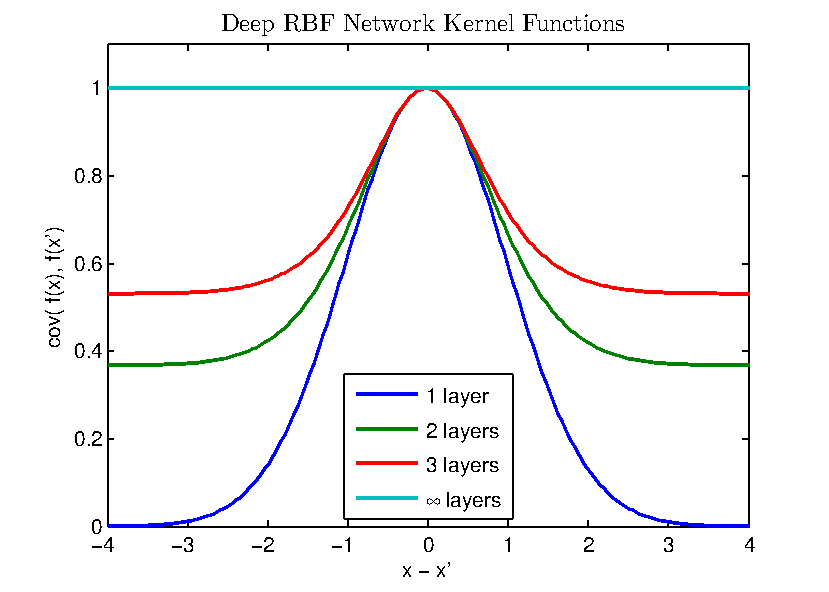
\includegraphics[width=0.33\columnwidth, clip, trim = 0cm 0cm 1cm 0.61cm]{../figures/deep_kernel} &
Deep connected kernel \\
\hspace{-0.5cm}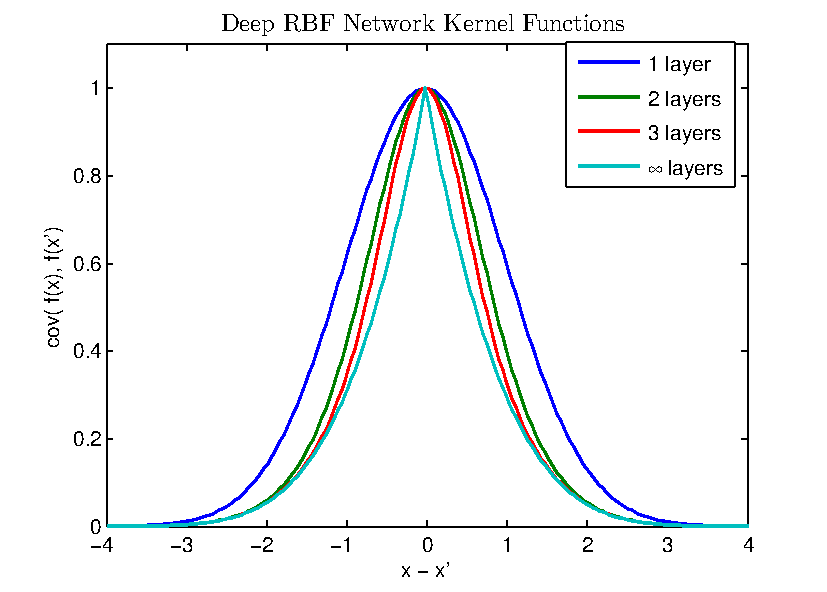
\includegraphics[width=\columnwidth, clip, trim = 0cm 0.4cm 0.9cm 0.3cm]{../figures/deep_kernel_connected}
% \\
%Connected \gp{} draws \\
%\hspace{-0.5cm}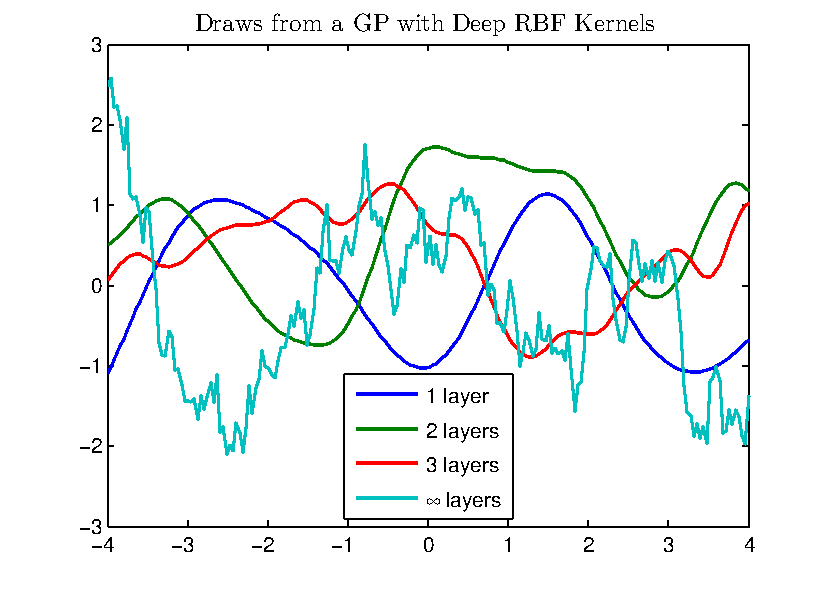
\includegraphics[width=\columnwidth, clip, trim = 0cm 0.1cm 0.9cm 0.35cm]{../figures/deep_kernel_connected_draws}
\end{tabular}
\end{centering}
\end{minipage}








\mysection{Conclusions}


%\raggedright

\begin{tabular}{cc}
\begin{minipage}[c]{0.8\columnwidth}

\begin{itemize}
	\item Random networks capture fewer degrees of freedom as they get deeper
	\item Connecting the input to each layer resolves this pathology
%	\item Deep Gaussian processes are a data-independent way to characterize neural networks
%	\item Deep One-Dimensional \gp{}s have a log-normal distribution on the magintude of their derivatives.
	\item Can build arbitrarily deep kernels
\end{itemize}

Code at \texttt{github.com/duvenaud/deep-limits}

Paper at \texttt{mlg.eng.cam.ac.uk/duvenaud/papers/verydeep.pdf}

\end{minipage}
&
\begin{minipage}[c]{0.2\columnwidth}
\begin{centering}

\includegraphics[width=\linewidth]{figures/qrcode-paper-link}
\end{centering}
\end{minipage}
\end{tabular}
%
%
%
